%!TEX root = ../dissertation.tex

\chapter{Tangram extensions for analysis}
\label{appendix:more-tangram}

\section{Interaction analysis}
% \addcontentsline{toc}{subsection}{Interaction analysis}
\subsection{GaudiView}
% \addcontentsline{toc}{subsubsection}{GaudiView}
GaudiMM, described in \autoref{chap:04}, can generate tens of solutions including several ‘good-enough’ answers to the problem posed due to its multi-objective nature. Seeing them all in UCSF often meant waiting for all the files to load beforehand, even the ones you might not be interested in seeing. Additionally, hiding the current one to show the following one required more than one action. As a result, the GaudiView graphical interface was designed to overcome those difficulties by providing the following features:

\begin{itemize}
	\item Provide a tabular view of the results listing all the solutions in rows, and objective scores in columns. Rows can be sorted by one or more columns and filtered out by providing one or more cutoffs depending on the value of one column.

	\item Since the result index (\texttt{$\ast$ .gaudi-output} file) already contains the list of filenames and their scores, this is enough to display the initial table. Actual molecule objects are only loaded when its row is selected. This allows for fast browsing of only the requested solutions, without initial loading times.

	\item Every time one or more new rows are selected (with a mouse click or with keyboard arrows), the previously selected rows are hidden and the new ones are displayed.

	\item New selections can run any Chimera command specified in the command-line field below the table. This can be really useful to update the displayed residues around a ligand in protein-ligand docking, for example.

	\item Some clustering and rescoring utilities are also included for deeper analysis.
\end{itemize}

The architecture behind GaudiView does not depend on the initial data structure: a preprocessing step is performed to build the tabular data view, that ultimately servers molecules to the interactive canvas. Thanks to that, it’s easy to integrate other file formats that can benefit from this interface. Currently, GaudiView accepts solutions from GOLD and arbitrary lists of Mol2 files. In the future, more docking programs could be integrated, like AutoDock Vina or DOCK.

\subsection{NCIPlotGUI}
% \addcontentsline{toc}{subsubsection}{NCIPlotGUI}
NCIPlot is a widely used visualization method developed by Contreras-García et al\cite{nciplot} that uses non-covalent interaction indices derived from electronic density and its derivatives (\todo{CHECK XXX}) to help distinguish attractive interactions like Van der Waals, London dispersion forces or hydrogen bonds from repulsive ones like bad steric impediments. The original implementation is a FORTRAN program that requires specific input file with atomic coordinates and special keywords. While not difficult to write, it is still a small entry barrier.

With NCIPlotGUI, the input file is automatically generated from any opened molecule in UCSF Chimera and the calculation is run in the background. When the program is done, the results are loaded in the same UCSF Chimera instance and plotted as colored volume maps (see fig. \ref{fig:tangram-nciplot}). For large numbers of atoms, an alternative, 40-times faster CUDA implementation of the NCIPlot method\cite{nciplotcuda} is also supported and recommended for GPU-enabled computers.



\begin{figure}
	\begin{Center}
		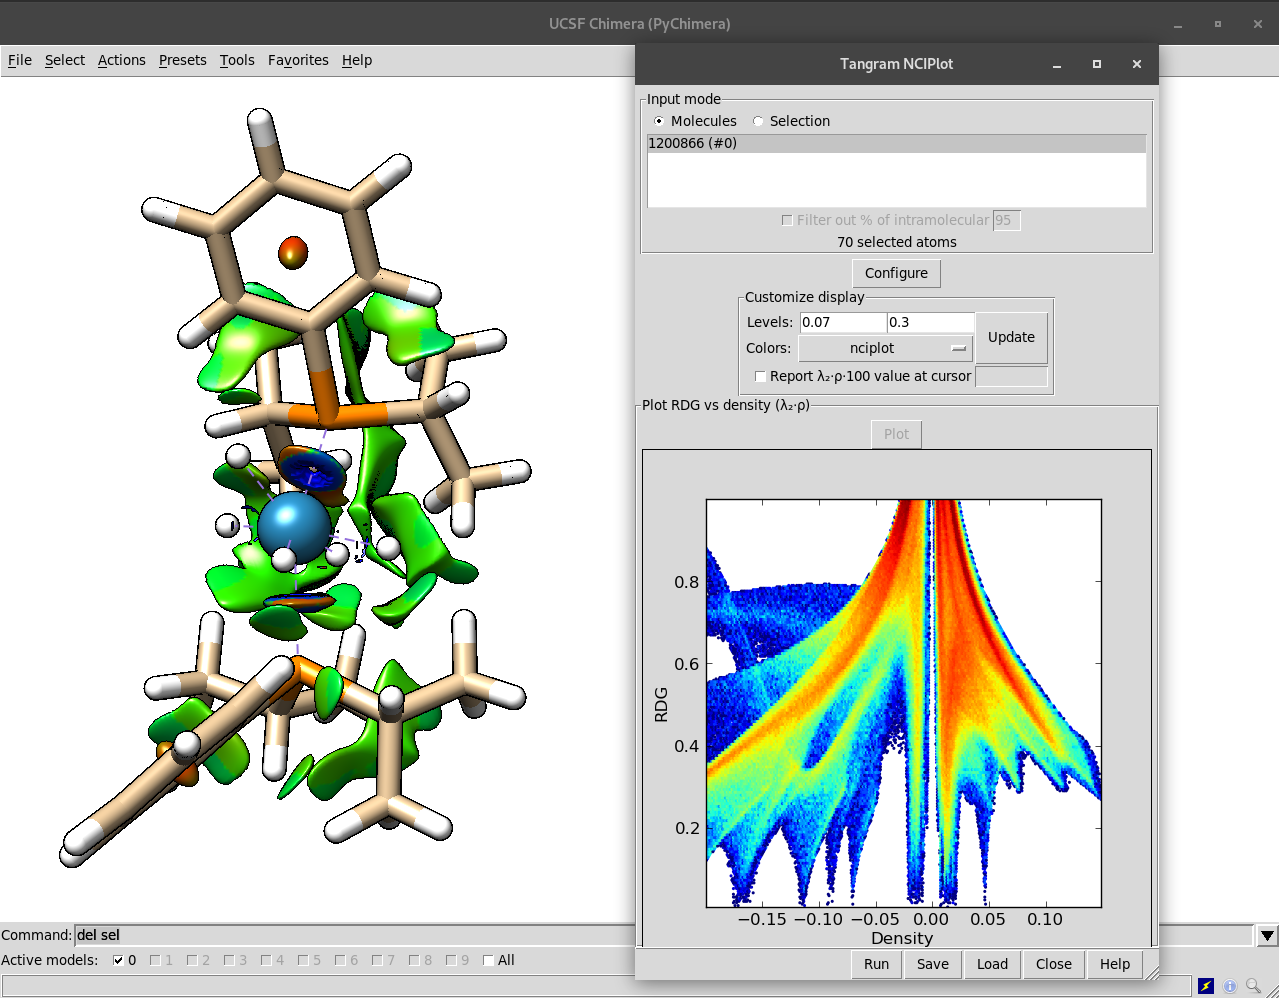
\includegraphics[width=\textwidth]{./figures/05/tangram_nciplot.png}
		\caption[Tangram NCIPlotGUI]{Non-Covalent Interaction analysis of the partial structure of KUJLIK CSD structure $ \{ $ $ \} $ , with 70 atoms. The interface shows the input and configuration forms, as well as the Reduced Density Gradient (RDG) versus Density plot}
		\label{fig:tangram-nciplot}
	\end{Center}
\end{figure}

\subsection{PLIPGUI}
% \addcontentsline{toc}{subsubsection}{PLIPGUI}
Protein-Ligand Interaction Profiler (PLIP)\cite{salentin2015plip} is a Python utility to identify, list and represent non-covalent interactions between protein-ligand complexes. It depends on OpenBabel and VMD to work, but some UCSF Chimera integration is available. PLIPGUI is a Chimera extension that wraps PLIP in a graphical interface so all the tasks can be performed in a single program. The resulting will list all the identified interactions with a dynamic table that is updated depending on the binding site selected (if multiple are present). This can be coupled with docking studies to identify additional features implicitly described in the docking score.\footnote{For example, in GaudiView, the included \texttt{plip} command can be run for each solution, illustrating the possible cooperative tasks enabled with Tangram.}

\section{Structure analysis}
% \addcontentsline{toc}{subsection}{Structure analysis}

\subsection{3D-SNFG}
% \addcontentsline{toc}{subsubsection}{3D-SNFG}
Glycoproteins are proteins that feature oligosaccharidic cofactors and are actively researched for its involvement in recognition processes, metabolism and allergies. However, since they are essentially different variations or 6 or 5-member alkane rings with hydroxyl \todo{(or some other functional groups?)} substitutions, it is difficult to differentiate them visually when using classic 2D or 3D depictions. For that reason, the GLYCAM committee decided on a standardized 2D representation using colored geometric shapes called Symbol Nomenclature for Glycans (SNFG).\cite{snfg} A 3D implementation for VMD was developed by Thieker et al\cite{3dsnfg} in TCL language, and is the original 3D-SNFG project. This is a reimplementation of the same idea, but using Python and UCSF Chimera. It provides three alternative depictions, and the possibility to customize sizes and scales without modifying the source code (as it was expected in the original TCL implementation). The representation (see fig. \ref{fig:tangram-snfg}) can be switched on with the \texttt{snfg} command and switched off with \texttt{$ \sim $ snfg}.

\begin{figure}[t]
	\begin{Center}
		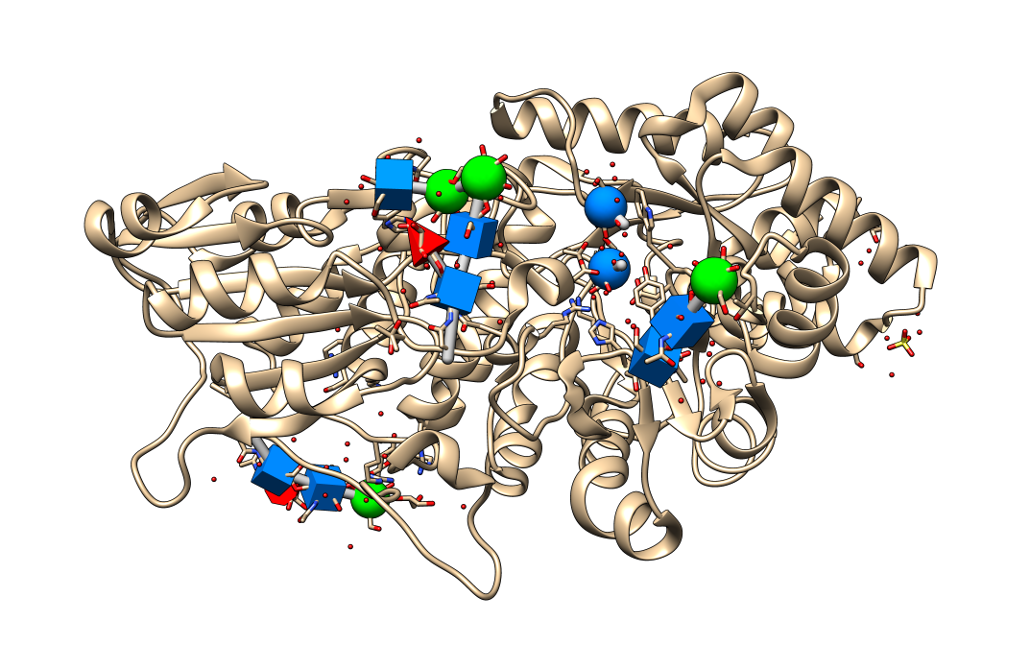
\includegraphics[width=\textwidth]{./figures/05/tangram_snfg.png}
	\end{Center}
	\cprotect\caption[Tangram 3D-SNFG]{3D-SNFG representation of glycoside exohydrolase from \textit{Hordeum vulgare}.\cite{3wlh}}
	\label{fig:tangram-snfg}
\end{figure}

\subsection{BondOrder}
% \addcontentsline{toc}{subsubsection}{BondOrder}
UCSF Chimera does not consider bond orders in the connectivity information it stores or represents. An approximate calculation is done during the parsing stage of molecule files to compute some internal atom types, but then that data is discarded. For some jobs, this information is important, though.

This extension provides a way to define an ‘order’ parameters manually in chimera.Bond objects, so it can be used by other extensions that could rely on it. For example, QMSetup could use it to write the connectivity matrix using proper bond orders instead of the default 1.0. When the order attribute is present, this extension enables alternative representations of the bond with additional decorations in the cylinder.

Additionally, the bond order information can be automatically computed with external libraries like RDKit, OpenBabel or AmberTools. The algorithms employed in that case are only applicable for small molecules though, so some work is needed when dealing with macromolecules. In those cases, template structures for common residues could be applied.

\subsection{OrbiTraj}
% \addcontentsline{toc}{subsubsection}{OrbiTraj}
OrbiTraj patches the Molecular Dynamics trajectory viewer already present in Chimera and adds support for loading volume files for each frame. For example, this can be useful for QM optimization calculations where orbitals data have been generated for each frame. By using the OrbiTraj patch, the XYZ trajectory can display the orbitals volumetric isosurfaces along the way, thus representing electronic density transfer. The package also ships some independent Python scripts that can be used to convert WFN files as provided by Gaussian to CUBE files compatible with UCSF Chimera loaders.


\subsection{PoPMuSiCGUI}
% \addcontentsline{toc}{subsubsection}{PoPMuSiCGUI}
PoPMuSiC\cite{dehouck2011popmusic} is a web service that can calculate potentially stabilizing mutation sites in protein and peptide structures. Users need to register an account before submitting their files, and once the results are computed, they can be download from the user web panel. The results are plain-text files that list the different mutations associated to each residue position and their calculated score. PoPMuSiCGUI can open these files along with the submitted protein structure and depict those scores in a dynamic, two-panel tabular view. Residues can be colored according to is ‘mutability’ score: positions that would stabilize under certain mutations will have a positive score and colored in a shade of green proportional to that score, while non-stabilizable positions would have a negative score and a red shade. Additionally, residue positions can be mutated to one of the proposed substitutions by using the Dunbrack's\cite{dunbrack1993backbone} and Dynameomics\cite{scouras2011dynameomics} rotamer libraries implemented in UCSF Chimera, which will have the changes immediately applied in the interactive 3D canvas.



\begin{figure} % FIXME!
	\begin{Center}
		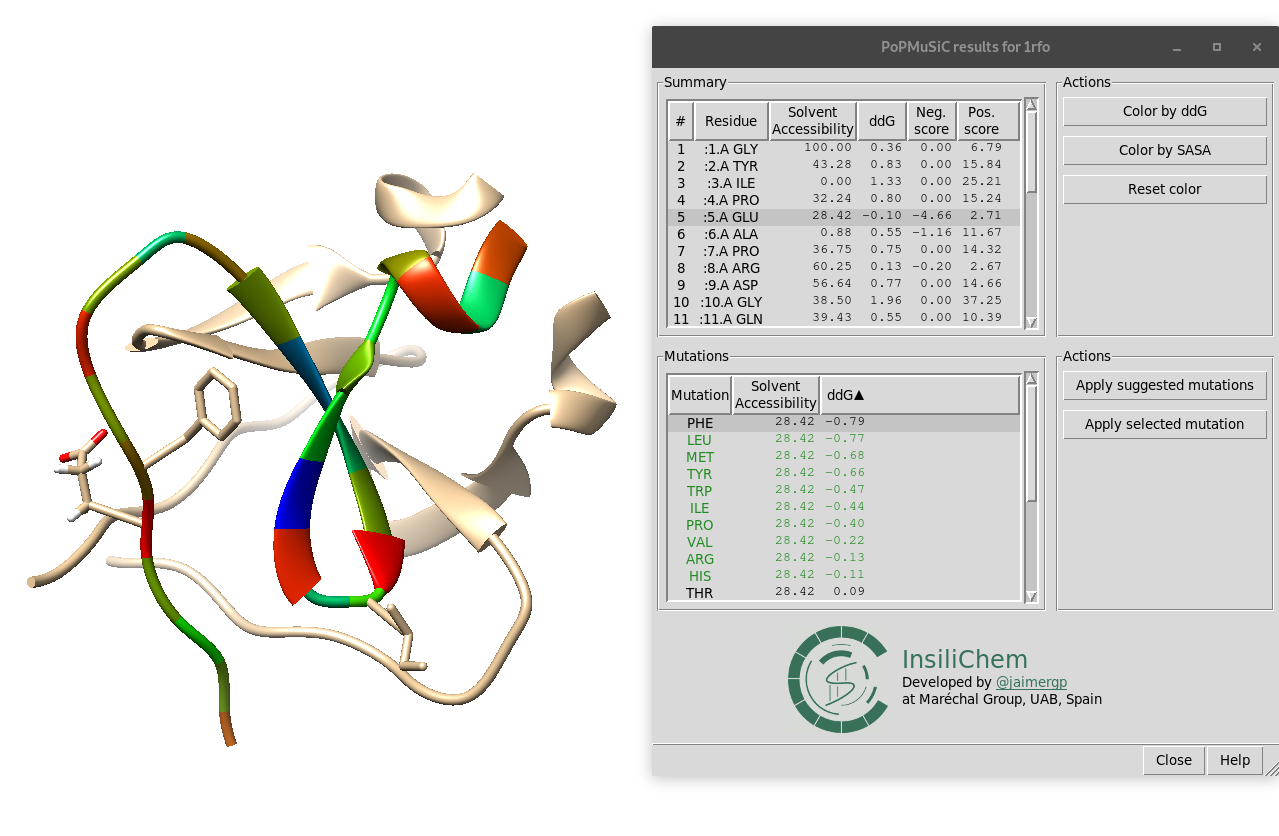
\includegraphics[width=\textwidth]{./figures/05/tangram_popmusic.png}
	\end{Center}
	\cprotect\caption[Tangram PoPMuSiC GUI]{PoPMuSiC results for the trimeric Foldon of the T4 phagehead fibritin.\cite{1rfo} One of the monomers has been colored according to the stabilizing potential of a mutation in that position (red being destabilizing, green neutral, and blue stabilizing).}
	\label{fig:tangram-popmusic}
\end{figure}


\subsection{PropKaGUI}
% \addcontentsline{toc}{subsubsection}{PropKaGUI}
PropKa is a Python library developed by Jensen\cite{propka}  that calculates pKa values of protein residues under different environment pH values. PropKaGUI wraps this package to make it usable in UCSF Chimera with a simple graphical interface. After selecting the opened molecule to be analyzed and the pH value, the PropKa routines are run and the results are shown in a new dialog listing the calculated pKa value for each residue. \todo{Adequate hydrogens can be added in situ by taking that information into account.}

\subsection{SubAlign}
% \addcontentsline{toc}{subsubsection}{SubAlign}
UCSF Chimera provides several utilities for molecular superposition. The ‘matchmaker’ command allows to efficiently superpose protein structures using sequence alignment and homology score matrices as guiding criteria. For non-protein structures, the simple ‘match’ command is able to obtain the optimal superposition of two molecules, but only if atom pairs correspondences are manually provided. Several algorithms exist to identify the best atoms correspondences automatically,\cite{cho2006flame,girones2001tgsa} but none of them are implemented in Chimera. The SubAlign extension provides a command (no graphical interface currently) to superpose small molecules by applying several alignment protocols implemented in RDKit.\cite{rdkit} The root-mean-square deviation (RMSD) of the superposed molecules is also provided as a result of the alignment, so it can be used for that kind of analysis as well. If more than two molecules are provided, all of them are aligned against the first, and the average RMSD is reported. In the future, more algorithms can be implemented, with a particular focus on those coming from the Computer Vision field, where Point Set Registration problems are common.
